%\usepackage{CJK}
 %必需在Xelatex下才行
\documentclass[UTF8]{ctexart}
%\setCJKmainfont{FZYaoTi}  %宋体
\usepackage{amsmath}
\usepackage{cite}
\usepackage{graphicx}
\usepackage{geometry}
\geometry{papersize={21.0cm,29.7cm}}
\geometry{left=1cm,right=2cm,top=3cm,bottom=4cm}

\usepackage{setspace}
\onehalfspacing    %行间距
\addtolength{\parskip}{.4em}  %段间距增加0.4
\usepackage{float}

\title{地球流体动力学作业\\[2ex]\begin{large} QBO推导与重复 \end{large} }
\author{李洋}
\date{\today}

\usepackage{fancyhdr}
\pagestyle{fancy}
%\pagestyle{plain}
\lhead{\author{李洋}}
%\chead{\date{\today}}
\rhead{地球流体动力学作业}
\lfoot{}
\cfoot{\thepage}
\rfoot{}
\renewcommand{\headrulewidth}{0.4pt}
\renewcommand{\headwidth}{\textwidth}
\renewcommand{\footrulewidth}{0pt}
\begin{document}
	 %\tableofcontents  %目录
	\maketitle
	\section{模型简述}
	Holton \& Lindzen(1972)通过底层向上传播Kelvin波与mixed gravity-Rossby波的扰动,
	与顶层半年循环的平均流强迫相互作业,模拟了一个准两年的东西风震荡。
	
	Kelvin波与mixed gravity-Rossby波对平均流东西风的贡献,及其被平均流吸收的条件
	有很大不同。Kelvin波向上传递西风分量,本身相速度也向东。当基本气流是东风时,
	Kelvin波容易上传,使基本气流逐渐转为西风;但当西风较强,风速与波速接近时,
	Kelvin波的扰动很难再传上去。
	另一方面,mixed gravity-Rossby波向上传递东风分量,本身相速度也向西。当东风较强,
	风速与波速接近时,扰动很难再传上去。
	这两种波配合高空的半年循环产生了QBO现象。
	\section{推导摘要}
	\subsection{基本方程}
	基本态满足:
	\[\beta yU=-\frac{1}{\rho_0}\frac{\partial p_0}{\partial y}\]
	\[\frac{\partial p_0}{\partial z}=-\rho_0g\]
	若基本气流只是高度的函数,则能推出:
	\[ln\rho_0=\frac{1}{2}\frac{\beta y^2}{g}\frac{dU}{dz}+F(z)\]
	这里取$F(z)=-Sz$,即密度指数衰减。
	
	进一步,如果扰动采取东西方向的行波解的形式,扰动方程可写作:
	\[i\widehat{\omega}u+w\frac{dU}{dz}=-ik\Phi+\beta yv\]
	\[i\widehat{\omega}v=-\frac{\partial\Phi}{\partial y}-\beta yu\]
	\[\frac{\partial \Phi}{\partial z}=-g\frac{\delta\rho}{\rho_0}\]
	\[i\widehat{\omega}\frac{\delta\rho}{\rho_0}-wS+\frac{\beta y}{g}\frac{dU}{dz}v=0\]
	\[iku+\frac{\partial v}{\partial y}+\frac{\partial w}{\partial z}=0\]
	其中
	\[\widehat{\omega}=\omega +kU-i\alpha\]
	\[\Phi=\frac{\delta p}{\rho_0}\]
	
	忽略$O\{(\frac{dU}{dz})^2/(gS)\}$项,可以得到关于单一变量$\Phi$的方程:
	\begin{align} \label{eq1}
	\nonumber(\beta^2y^2-{\widehat{\omega}}^2)^2\frac{\partial^2\Phi}{\partial z^2}+
	2\beta y(\beta^2y^2-{\widehat{\omega}}^2)\frac{dU}{dz}
	\frac{\partial^2\Phi}{\partial z\partial y}+gS[(\beta^2y^2-{\widehat{\omega}}^2)
	\frac{\partial^2\Phi}{\partial y^2}+\beta\frac{dU}{dz}[\frac{\beta y^2}{gS}
	(\beta^2y^2-{\widehat{\omega}}^2)\frac{dU^2}{dz^2}-(\beta^2y^2+{\widehat{\omega}}
	^2)]\frac{\partial\Phi}{\partial z}\\-2gS\beta y^2\frac{\partial\Phi}{\partial y}+
	\frac{gSk}{\widehat{\omega}}[\beta(\beta^2y^2+{\widehat{\omega}}^2)-k\widehat
	{\omega}(\beta^2y^2-{\widehat{\omega}}^2)]\Phi=0\
	\end{align}
	
	将上述方程中的y与z进行变量替换,即:
	\[\tau=\epsilon z, \epsilon\ll1\]
	\[\widehat{z}=\int_0^zf(\tau)dz\]
	\[\xi=y/l(\tau)\]
	\[l=l_0(\tau)+\epsilon l_1(\tau)+\cdots\]
	
	此时令
	\[\Phi=\Phi_0(\widehat{z},\tau,\xi)+\epsilon\Phi_1(\widehat{z},\tau,\xi)+\cdots\]
	带入(\ref{eq1})得到关于$\epsilon$的0阶方程为\footnote{Lindzen (1971)\cite{deduct}里对应这个公式的(23)
		以及后面的1阶方程(36)都有写错的地方,从量纲即可看出}:
	\begin{align} \label{eq2}
	(\beta^2\xi^2l_0^2-{\widehat{\omega}}^2)^2f^2\frac{\partial^2\Phi_0}{\partial \widehat{z}^2}+\frac{gS}{l_0^2}
	(\beta^2\xi^2l_0^2-{\widehat{\omega}}^2)^2\frac{\partial}{\partial\xi}[\frac{1}{\beta^2\xi^2l_0^2-
	{\widehat{\omega}}^2}\frac{\partial\Phi_0}{\partial\xi}]+\frac{gSk}{\widehat{\omega}}[\beta(\beta^2\xi
	^2l_0^2+{\widehat{\omega}}^2)-k\widehat{\omega}(\beta^2\xi^2l_0^2-{\widehat{\omega}}^2)]\Phi_0=0
	\end{align}
	对不同的n,这个方程都能得到\footnote{这里没看懂}:
	\begin{align}\label{sup}
	\beta^2l_0^4=\frac{gS}{f^2}=gh^{(n)}
	\end{align}
	关于$\epsilon$的1阶方程为:
	\begin{align} \label{eq3}
	\nonumber\frac{f^2l_0^2}{gS}\frac{\partial^2\Phi_1}{\partial \widehat{z}^2}+
	\frac{\partial}{\partial\xi}[\frac{1}{\beta^2\xi^2l_0^2-{\widehat{\omega}}^2}
	\frac{\partial\Phi_1}{\partial\xi}]+\frac{l_0^2k}{\widehat{\omega}}[\beta\frac{(\beta^2\xi
	^2l_0^2+{\widehat{\omega}}^2)}{(\beta^2\xi^2l_0^2-{\widehat{\omega}}^2)^2}-k\widehat{\omega}
	\frac{1}{(\beta^2\xi^2l_0^2-{\widehat{\omega}}^2)}]\Phi_1=\\
	-\frac{l_0^2}{gS}[I_1+\frac{I_2}{(\beta^2\xi^2l_0^2-{\widehat{\omega}}^2)}+\frac{I_3}
	{(\beta^2\xi^2l_0^2-{\widehat{\omega}}^2)^2}]
	\end{align}	
	其中,$I_1,I_2,I_3$与$\Phi_0$与$l_1$相关。
	\subsection{Kelvin波波流相互作业推导}
	以下部分仅针对n=-1\footnote{n的选择见\cite{n}},即Kelvin波进行推导,Yanai波(n=0)同理。
	\[\Phi_0^{(-1)}=A_0^{(-1)}(\tau)exp(-\xi^2/2)exp(i\widehat{z})\]
	\begin{align}\label{sup2}
		\sqrt{gh^{(-1)}}=-\frac{\widehat{\omega}}{k}
	\end{align}
	方程(\ref{sup2})相对于没有牛顿冷却项的c加了一个虚数的部分$i\frac{\alpha}{k}$
	
	方程(\ref{eq3})左侧与(\ref{eq2})是形式是相同的。这时应该考虑两个条件:
	
	1. 如果方程(\ref{eq3})右侧的项与$\Phi_0$成比例,这
	对$\Phi_1$相当于给了一个共振频率的外强迫,会引起共振。
	
	2. 当$\beta^2\xi^2l_0^2-{\widehat{\omega}}^2=0$
	时,右侧第二项与第三项都是奇点,对应无限的强迫。至少应该要求,这两项对整个y(或$\xi$)积分应该是有限的。
	所以,被积分项最大只能有一阶极点,因此要求
	\[I_3\propto\beta^2\xi^2l_0^2-{\widehat{\omega}}^2\]
	
	此时恰巧右侧第二项与第三项之和为0,让第一项对$\xi$的积分对$\Phi_0$无投影来避免共振,最后得到
	\[A_0=\frac{constant}{\sqrt{fl_0}}\]
	这样,记
	\[-\frac{\widehat{\omega}}{k}\equiv c-U\]
	由方程(\ref{sup}、\ref{sup2})可知,$f\propto\frac{1}{c-U}$,$l_0\propto(c-U)^{\frac{1}{2}}$,
	从而
	\[\Phi_0\propto(c-U)^{\frac{1}{4}}exp(i\widehat{z})\]
	\[w_0\propto(c-U)^{\frac{1}{4}}exp(i\widehat{z})\]
	\[u_0\propto(c-U)^{-\frac{3}{4}}exp(i\widehat{z})\]
	\[v_0=0\]
	所以,记$\left\langle\ \right\rangle$为对y积分,$\bar{\ }\ $代表对时间或纬向平均
	\begin{align}\label{flux}
	\left\langle\bar{F}/\rho\right\rangle=\left\langle{\overline{u_0w_0}}\right\rangle\propto
	\frac{1}{(c-U)^{1/2}}\frac{dy}{d\xi}\int_{-\infty}^{+\infty}exp(-\xi^2)d\xi\ exp(2i\widehat{z})
	=Aexp(2i\ Im\{\widehat{z}\})
	\end{align}
	为了求$\widehat{z}$的虚部,将f中的$i\frac{\alpha}{k}$恢复出来,c恢复为$-\frac{\omega}{k}$,泰勒展开得到
	\begin{align}\label{f}
	f^{(-1)}\approx\frac{\sqrt{gS}}{c-U}[1-\frac{i\alpha}{k(c-U)}]
	\end{align}
	因此,Kevin波水平动量的垂直输送是
	\[Aexp(-2\int_{0}^{z}g_0(z)dz)\]
	\[ g_0=\frac{1}{2}\frac{\sqrt{gS}}{(c-U)^2}\frac{\alpha}{k}
	\]
	
	如果带入具体的比例可知Kelvin波的通量恒为正(Yanai恒为负)。至此,全部需要的方程都以推导完毕。
	\section{数值重复}
	采用与Holton and Lindzen(1972)\cite{main}同样的参数以及分辨率(250m,24hr),垂直差分采用中央差,垂直
	积分采用梯形近似,时间上采取最普通的欧拉前向积分。对$c-U$的绝对值加一个下界(0.002m/s)以防止超出数值范围。
	得到的结果图()所示,确实存在东西风的
	准两年变化,这与Holton and Lindzen(1972)\cite{main}的结果一致。
	\begin{figure}[H]
		\centering
		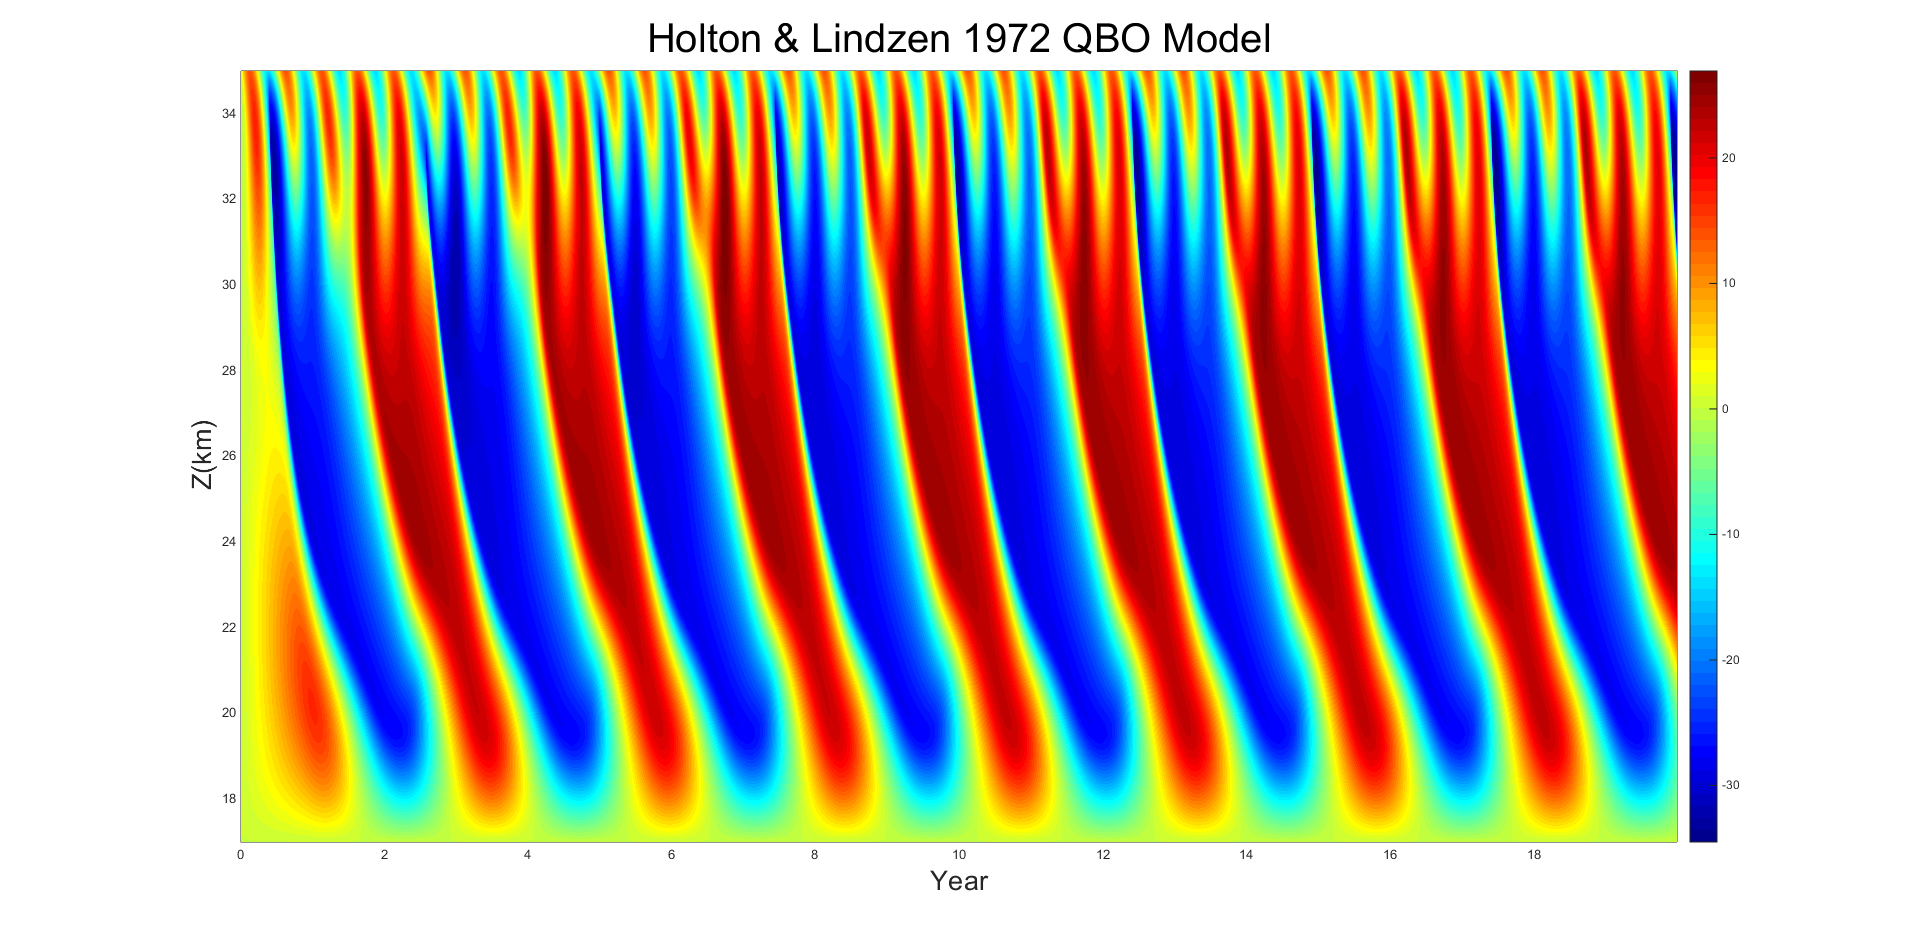
\includegraphics[height =.3\textheight]{qbo.png}
		\caption{QBO模拟}
		\label{fig:delta18000}
	\end{figure}
	
	
	

\begin{thebibliography}{99}
	\bibitem{deduct} Lindzen, Richard S. "Equatorial planetary waves in shear. Part I." Journal of the Atmospheric Sciences 28.4 (1971): 609-622.
	\bibitem{n} Holton, James R., and Richard S. Lindzen. "A note on Kelvin waves in the atmosphere." Mon. Wea. Rev 96 (1968): 385-386.
	\bibitem{main} Holton, James R., and Richard S. Lindzen. "An updated theory for the quasi-biennial cycle of the tropical stratosphere." Journal of the Atmospheric Sciences 29.6 (1972): 1076-1080.
\end{thebibliography}
\end{document}